% !TEX encoding = ISO-8859-1
\documentclass[bsc,oneside]{ufpethesis}

% \usepackage[T1]{fontenc}

\usepackage{amssymb}
\usepackage{amsmath}
\usepackage{mathtools}
\usepackage{hyperref}
\usepackage{algorithm}
\usepackage{algorithmic}
\usepackage{subfigure}
\usepackage{appendix}

\algsetup{linenosize=\small,linenodelimiter=.}
\hypersetup{colorlinks,citecolor=black,filecolor=black,linkcolor=black,urlcolor=black}

\usepackage{amsthm}

% \university{<NOME DA UNIVERSIDADE>} default: UFPE
% \address{<CIDADE DA IES>} default: UFPE
\institute{Centro de Inform�tica}
% \department{<NOME DO DEPARTAMENTO>} n�o se aplica
\program{Gradua��o em Engenharia da Computa��o}
\majorfield{Engenharia da Computa��o}
\title{An�lise comparativa de t�cnicas de sele��o de prot�tipos}
\date{22 de novembro de 2011}

\author{Dayvid Victor Rodrigues de Oliveira}
\adviser{Prof. Dr. George Darmiton}
% \coadviser{NOME DO(DA) CO-ORIENTADOR(A)} n�o se aplica

%% Inicio do documento
\begin{document}

\frontmatter
% Folha de rosto
\frontpage
% Portada (apresenta��o)
\presentationpage

% Dedicat�ria
\begin{dedicatory}
Eu dedico este trabalho a Jo�o Rodrigues de Silva, meu av�.
\end{dedicatory}

% Agradecimentos
\acknowledgements
Agrade�o a Deus.
% % !TEX encoding = ISO-8859-1

Agradeço a Deus.



\begin{epigraph}[Boston, 2001]{Bono}
What can I give back to God, for the blessings You pour out on me?
\end{epigraph}

% Resumo em Portugu�s
% Se preferir, crie um arquivo � parte e o inclua via \include{}
\resumo
RESUMO
% Palavras-chave do resumo em Portugu�s
\begin{keywords}
PORTUGUES
\end{keywords}

% Resumo em Ingl�s
% Se preferir, crie um arquivo � parte e o inclua via \include{}
\abstract
ABSTRACT
\begin{keywords}
INGLES
\end{keywords}

\tableofcontents
\listoffigures
\listoftables

\mainmatter




the introdution goes here \cite{cnn:1968}.

% !TEX encoding = ISO-8859-1
\chapter{T�cnicas de Sele��o de Prot�tipos}
% \label{ch:introducao}

Neste cap�tulo, ser�o mostradas as t�cnicas de sele��o de prot�tipos abordadas neste trabalho. Cada uma das sess�es abaixo abordar� uma t�cnica, ser� mostrado o conceito da t�cnica, assim como o pseudo-c�digo e as caracter�sicas de cada uma destas t�cnicas.

\section{ENN}

	Edited Nearest Neighbor Rule\cite{enn:2011} � uma t�cnica de sele��o de prot�tipos puramente seletiva proposta por Wilson em 1976. De uma forma geral, esta t�cnica foi projetada para funcionar como um filtro de ru�dos, ela elimina pontos na regi�o de fronteira, regi�o de alta susceptibilidade a erros, e com isso elimina ru�dos.
	Por atuar apenas na regi�o de fronteira, esta t�cnica possui uma baixa capacidade de redu��o, deixando as inst�ncias que n�o se encontram na regi�o de fronteira intactas, exceto pelos ru�dos extremos.
	Uma desvantagem desta t�cnica � que ela possui uma baixa capacidade de redu��o de elementos, visto que ela n�o elimina redund�ncia.

	Segue abaixo o algor�tmo da execu��o do ENN e, logo ap�s, alguns coment�rios sobre este algor�tmo.



\section{Tomek Links}
\section{CNN}
\section{LVQ}
\subsection{LVQ 1}
\subsection{LVQ 2.1}
\subsection{LVQ 3}
\section{SGP}
\section{SGP 2}
\section{CCNN}



% !TEX encoding = ISO-8859-1
\chapter{An�lise em Bases Artificiais}
\label{ch:analiseembasesartificiais}

Neste cap�tulo ser� analisado o desempenho das t�cnicas acima em bases desbalanceadas artificiais. Al�m da taxa de acerto, ser� considerada a quantidade de prot�tipos gerados por cada t�cnica e a distribui��o destes prot�tipos.

\section{Bases Artificiais}
\label{sec:basesartificiais}

Para avaliar de forma visual o comportamento de cada algoritmo de sele��o de prot�tipos, foram selecionadas bases artificiais com diferentes n�veis de sobrebosi��o entre a classe marjorit�ria e a classe minotir�ria. Tamb�m foram selecionados dois diferentes n�veis de desbalanceamento, um com aproximadamente 10\% de desbalanceamento e outro com aproximadamente 5\%.

\begin{figure}[H]
\center
\includegraphics[scale=0.40]{imagens/outputs/ORIG_10_0.eps}
\caption{Base Original com 10\% de desbalanceamento e intersec��o m�nima}
\label{fig:orig1}
\end{figure}

\begin{figure}[H]
\center
\includegraphics[scale=0.40]{imagens/outputs/ORIG_10_15.eps}
\caption{Base Original com 10\% de desbalanceamento e intersec��o m�xima}
\label{fig:orig2}
\end{figure}


Nas figuras \ref{fig:orig1} e \ref{fig:orig2} est�o demonstrados os n�veis de intersec��o extremos. No primeiro caso, a classe marjorit�ria est� totalmente separada da classe minorit�ria. No segundo caso, a classe marjorit�ria engloba toda a classe minorit�ria. Al�m destes dois casos, tamb�m ser�o mostrados n�veis intermedi�rios de sobreposi��o. Com estes diferentes n�veis de intersec��o, ser� poss�vel avaliar o comportamento de cada t�cnica diante de diferentes casos de bases desbalanceadas.

\begin{figure}[H]
\center
\includegraphics[scale=0.40]{imagens/outputs/ORIG_5_0.eps}
\caption{Base Original com 5\% de desbalanceamento e intersec��o m�nima}
\label{fig:orig3}
\end{figure}

\begin{figure}[H]
\center
\includegraphics[scale=0.40]{imagens/outputs/ORIG_5_15.eps}
\caption{Base Original com 5\% de desbalanceamento e intersec��o m�xima}
\label{fig:orig4}
\end{figure}

Nas figuras \ref{fig:orig3} e \ref{fig:orig4} observa-se o mesmo caso, sendo que com um n�vel maior de desbalanceamento. Tendo as mesmas distribui��es e intersec��es, mas com n�veis de desbalanceamentos diferentes, ser� poss�vel avaliar a relev�ncia dos n�veis de desbalanceamento para cada t�cnica. 

\section{An�lise Individual}

Nesta sess�o, cada t�cnica sera analisada isoladamente. Para exemplificar e demonstrar as falhas de cada t�cnica, ser�o utilizadas figuras e tabelas que comprovem o comportamento de cada algoritmo diante de bases desbalanceadas.

Todas as conclus�es poder�o ser validadas ou mesmo reavaliadas com a aplica��o das t�cnicas de sele��o de prot�tipos em bases reais no pr�ximo cap�tulo.


\subsection{ENN}
\label{subsec:ennembasesartificiais}

	Conforme dito no cap�tulo anterior, o ENN � uma t�cnica que elimina ru�dos na fronteira de classifica��o, mantendo inst�ncias que apresentam redund�ncia de informa��o. Na tabela \ref{tab:enn5}, podemos ver a taxa de acerto do ENN em uma base com 10\%, onde o n�vel de sobreposi��o varia gradualmente, sendo o �ltimo n�vel o caso onda a classe minorit�ria est� totalmente imersa dentro da classe marjorit�ria, lembrando que, foi utilizado o pr�prio treinamento para teste, afim de avaliar a representatividade dos dados em rela��o a base original.

	Observa-se que a o ENN manteve uma boa taxa de acerto geral, sendo o pior caso com 94.74\%. Por�m, vemos que esta taxa diminui conforme o n�vel de sobreposi��o aumenta, na mesma propor��o em que inst�ncias s�o eliminadas. Por�m, ao observar a taxa de acerto da classe minorit�ria, pode-se perceber que o ENN eliminou muito mais inst�ncias da classe minorit�ria que da marjorit�ria.
	Inicialmente o n�vel de sobreposi��o das classes � zero, ent�o nenhuma inst�ncia � eliminada e a taxa de acerto � mantida. Conforme o n�vel de sobreposi��o das classes vai aumentnado, a taxa de acerto da classe minorit�ria vai decrescendo, chegando at� 0\% quando a classe minorit�ria est� totalmente sobreposta. Na tabela \ref{tab:enn10} acontece o mesmo, por�m, o decrescimento da taxa de acerto da classe minorit�ria � menor.


\begin{table}[H]
\begin{center}
\begin{tabular}{|l|l|l|l|l|l|}
\hline
N�vel de Intersec��o    &   I   &   II  &   III &   IV  &   V   \\
\hline %----- linha horizontal
Acerto total            &   100.00\%   &   100.00\%   &   97.68\%    &   94.74\%   &   94.74\%   \\
\hline
Acerto marjorit�ria     &   100.00\%   &   100.00\%   &   99.00\%    &   98.33\%   &   100.00\%   \\
\hline
Acerto minorit�ria      &   100.00\%   &   100.00\%   &   74.00\%    &   30.00\%   &   0.00\%   \\
\hline
Tamanho resultante      &   100.00\%   &   100.00\%   &   95.79\%    &   90.53\%   &   90.00\%   \\
\hline
\end{tabular}%--- fechamento do ambiente tabular
\end{center}   %fim da centraliza��o da tabela
\caption{ENN com n�vel de desbalanceamento 5\%}
\label{tab:enn5}
\end{table}


\begin{table}[H]
\begin{center}
\begin{tabular}{|l|l|l|l|l|l|}
\hline
N�vel de Intersec��o    &   I   &   II  &   III &   IV  &   V   \\
\hline %----- linha horizontal
Acerto total            &   100.00\%   &   100.00\%   &   95.80\%    &   90.00\%   &   90.00\%   \\
\hline
Acerto marjorit�ria     &   100.00\%   &   100.00\%   &   97.89\%    &   95.56\%   &   100.00\%   \\
\hline
Acerto minorit�ria      &   100.00\%   &   100.00\%   &   77.00\%    &   40.00\%   &   0.00\%   \\
\hline
Tamanho resultante      &   100.00\%   &   100.00\%   &   92.00\%    &   82.00\%   &   81.00\%   \\
\hline
\end{tabular}%--- fechamento do ambiente tabular
\end{center}   %fim da centraliza��o da tabela
\caption{ENN com n�vel de desbalanceamento 10\%}
\label{tab:enn10}
\end{table}


Quando n�o existe sobreposi��o de classes, o ENN pode ser uma boa op��o para remo��o de ru�dos, por�m, quando existe sobreposi��o, esta t�cnica pode remover praticamente todas as inst�ncias da classe minorit�ria, aumentando o n�vel de desbalanceamento e deixando o classificador invi�vel para identifica��o da classe minorit�ria.

\begin{figure}[H]
\center
\includegraphics[scale=0.40]{imagens/outputs/ENN_10_15.eps}
\caption{ENN sobre sobre base com total sobreposi��o de classes e 10\% de desbalanceamento}
\label{fig:enn1015}
\end{figure}

A figura \ref{fig:enn1015} mostra o que aconteceu ap�s a aplica��o do ENN. Todas as inst�ncias da classe minorit�ria foram removidas, pois foram tratadas como ru�dos. Apesar de inst�ncias da classe marjorit�ria tamb�m serem removidas, quanto maior o n�vel de desbalanceamento, mais invi�vel a t�cnica se torna, pois conforme a sobreposi��o aumenta, mais inst�ncias s�o removidas, e a classe minorit�ria tende a desaparecer mais rapidamente que a marjorit�ria.

Assim, tendo como base este experimento, conclui-se que o ENN n�o � uma t�cnica eficiente para se utilizar em bases altamente desbalanceadas, pois, quanto maior o n�vel de desbalanceamento, mais inst�ncias da classe minorit�ria ser�o eliminadas.

Uma poss�vel adapta��o do ENN seria remover inst�ncias apenas da classe marjorit�ria, com isso, o n�vel de desbalanceamento seria diminuido e a taxa de acerto da classe minorit�ria n�o seria afetada em rela��o ao KNN sobre toda a base original.


\subsection{CNN}

\begin{table}[H]
\begin{center}
\begin{tabular}{|l|l|l|l|l|l|}
\hline
N�vel de Intersec��o    &   I   &   II  &   III &   IV  &   V   \\
\hline %----- linha horizontal
Acerto total            &   94.74\%   &   99.26\%   &   97.47\%    &   94.74\%   &   94.11\%   \\
\hline
Acerto marjorit�ria     &   100.00\%   &   100.00\%   &   98.67\%    &   97.56\%   &   95.89\%   \\
\hline
Acerto minorit�ria      &   0.00\%   &   86.00\%   &   76.00\%    &   44.00\%   &   62.00\%   \\
\hline
Tamanho resultante      &   0.32\%   &   0.63\%   &   4.32\%    &   7.68\%   &   7.47\%   \\
\hline
\end{tabular}%--- fechamento do ambiente tabular
\end{center}   %fim da centraliza��o da tabela
\caption{CNN com n�vel de desbalanceamento 5\%}
\end{table}

\begin{table}[H]
\begin{center}
\begin{tabular}{|l|l|l|l|l|l|}
\hline
N�vel de Intersec��o    &   I   &   II  &   III &   IV  &   V   \\
\hline %----- linha horizontal
Acerto total            &   90.00\%   &   99.30\%   &   94.70\%    &   91.00\%   &   90.40\%   \\
\hline
Acerto marjorit�ria     &   100.00\%   &   99.44\%   &   96.22\%    &   94.44\%   &   95.00\%   \\
\hline
Acerto minorit�ria      &   0.00\%   &   98.00\%   &   81.00\%    &   60.00\%   &   49.00\%   \\
\hline
Tamanho resultante      &   0.50\%   &   1.20\%   &   7.50\%    &   13.30\%   &   13.90\%   \\
\hline
\end{tabular}%--- fechamento do ambiente tabular
\end{center}   %fim da centraliza��o da tabela
\caption{CNN com n�vel de desbalanceamento 10\%}
\end{table}

\subsection{Tomek Links}

\begin{table}[H]
\begin{center}
\begin{tabular}{|l|l|l|l|l|l|}
\hline
N�vel de Intersec��o    &   I   &   II  &   III &   IV  &   V   \\
\hline %----- linha horizontal
Acerto total            &   100.00\%   &   100.00\%   &   98.42\%    &   97.47\%   &   97.05\%   \\
\hline
Acerto marjorit�ria     &   100.00\%   &   100.00\%   &   99.33\%    &   98.67\%   &   99.00\%   \\
\hline
Acerto minorit�ria      &   100.00\%   &   100.00\%   &   82.00\%    &   76.00\%   &   62.00\%   \\
\hline
Tamanho resultante      &   100.00\%   &   100.00\%   &   96.84\%    &   94.32\%   &   94.32\%   \\
\hline
\end{tabular}%--- fechamento do ambiente tabular
\end{center}   %fim da centraliza��o da tabela
\caption{Tomek Links com n�vel de desbalanceamento 5\%}
\end{table}


\begin{table}[H]
\begin{center}
\begin{tabular}{|l|l|l|l|l|l|}
\hline
N�vel de Intersec��o    &   I   &   II  &   III &   IV  &   V   \\
\hline %----- linha horizontal
Acerto total            &   100.00\%   &   100.00\%   &   97.30\%    &   94.60\%   &   93.90\%   \\
\hline
Acerto marjorit�ria     &   100.00\%   &   100.00\%   &   98.56\%    &   97.00\%   &   97.56\%   \\
\hline
Acerto minorit�ria      &   100.00\%   &   100.00\%   &   86.00\%    &   73.00\%   &   61.00\%   \\
\hline
Tamanho resultante      &   100.00\%   &   100.00\%   &   94.60\%    &   89.60\%   &   89.60\%   \\
\hline
\end{tabular}%--- fechamento do ambiente tabular
\end{center}   %fim da centraliza��o da tabela
\caption{Tomek Links com n�vel de desbalanceamento 10\%}
\end{table}



\subsection{OSS}

\begin{table}[H]
\begin{center}
\begin{tabular}{|l|l|l|l|l|l|}
\hline
N�vel de Intersec��o    &   I   &   II  &   III &   IV  &   V   \\
\hline %----- linha horizontal
Acerto total            &   98.74\%   &   99.58\%   &   97.05\%    &   93.37\%   &   93.89\%   \\
\hline
Acerto marjorit�ria     &   98.67\%   &   99.56\%   &   97.11\%    &   93.44\%   &   94.22\%   \\
\hline
Acerto minorit�ria      &   100.00\%   &   100.00\%   &   96.00\%    &   92.00\%   &   88.00\%   \\
\hline
Tamanho resultante      &   5.58\%   &   5.89\%   &   7.16\%    &   8.63\%   &   9.68\%   \\
\hline
\end{tabular}%--- fechamento do ambiente tabular
\end{center}   %fim da centraliza��o da tabela
\caption{OSS com n�vel de desbalanceamento 5\%}
\end{table}

\begin{table}[H]
\begin{center}
\begin{tabular}{|l|l|l|l|l|l|}
\hline
N�vel de Intersec��o    &   I   &   II  &   III &   IV  &   V   \\
\hline %----- linha horizontal
Acerto total            &   97.50\%   &   98.80\%   &   95.20\%    &   85.90\%   &   87.50\%   \\
\hline
Acerto marjorit�ria     &   97.22\%   &   98.67\%   &   95.22\%    &   85.78\%   &   88.00\%   \\
\hline
Acerto minorit�ria      &   100.00\%   &   100.00\%   &   95.00\%    &   87.00\%   &   83.00\%   \\
\hline
Tamanho resultante      &   10.40\%   &   11.10\%   &   13.60\%    &   15.50\%   &   17.40\%   \\
\hline
\end{tabular}%--- fechamento do ambiente tabular
\end{center}   %fim da centraliza��o da tabela
\caption{OSS com n�vel de desbalanceamento 10\%}
\end{table}

\subsection{LVQ 1, 2.1 e 3}

\begin{table}[H]
\begin{center}
\begin{tabular}{|l|l|l|l|l|l|}
\hline
N�vel de Intersec��o    &   I   &   II  &   III &   IV  &   V   \\
\hline %----- linha horizontal
Acerto total            &   93.47\%   &   91.79\%   &   84.84\%    &   74.74\%   &   77.68\%   \\
\hline
Acerto marjorit�ria     &   93.11\%   &   91.33\%   &   84.00\%    &   73.33\%   &   76.44\%   \\
\hline
Acerto minorit�ria      &   100.00\%   &   100.00\%   &   100.00\%    &   100.00\%   &   100.00\%   \\
\hline
Tamanho resultante      &   1.05\%   &   1.05\%   &   1.05\%    &   1.05\%   &   1.05\%   \\
\hline
\end{tabular}%--- fechamento do ambiente tabular
\end{center}   %fim da centraliza��o da tabela
\caption{LVQ1 com n�vel de desbalanceamento 5\%}
\end{table}

\begin{table}[H]
\begin{center}
\begin{tabular}{|l|l|l|l|l|l|}
\hline
N�vel de Intersec��o    &   I   &   II  &   III &   IV  &   V   \\
\hline %----- linha horizontal
Acerto total            &   95.30\%   &   87.40\%   &   80.80\%    &   77.00\%   &   71.90\%   \\
\hline
Acerto marjorit�ria     &   94.78\%   &   86.00\%   &   78.67\%    &   74.44\%   &   68.78\%   \\
\hline
Acerto minorit�ria      &   100.00\%   &   100.00\%   &   100.00\%    &   100.00\%   &   100.00\%   \\
\hline
Tamanho resultante      &   1.00\%   &   1.00\%   &   1.00\%    &   1.00\%   &   1.00\%   \\
\hline
\end{tabular}%--- fechamento do ambiente tabular
\end{center}   %fim da centraliza��o da tabela
\caption{LVQ 1 acerto do 5 com n�vel de desbalanceamento 10\%}
\end{table}

\begin{table}[H]
\begin{center}
\begin{tabular}{|l|l|l|l|l|l|}
\hline
N�vel de Intersec��o    &   I   &   II  &   III &   IV  &   V   \\
\hline %----- linha horizontal
Acerto total            &   90.84\%   &   89.68\%   &   83.89\%    &   80.11\%   &   76.84\%   \\
\hline
Acerto marjorit�ria     &   90.33\%   &   89.11\%   &   83.00\%    &   79.00\%   &   75.56\%   \\
\hline
Acerto minorit�ria      &   100.00\%   &   100.00\%   &   100.00\%    &   100.00\%   &   100.00\%   \\
\hline
Tamanho resultante      &   1.05\%   &   1.05\%   &   1.05\%    &   1.05\%   &   1.05\%   \\
\hline
\end{tabular}%--- fechamento do ambiente tabular
\end{center}   %fim da centraliza��o da tabela
\caption{LVQ 2 com n�vel de desbalanceamento 5\%}
\end{table}

\begin{table}[H]
\begin{center}
\begin{tabular}{|l|l|l|l|l|l|}
\hline
N�vel de Intersec��o    &   I   &   II  &   III &   IV  &   V   \\
\hline %----- linha horizontal
Acerto total            &   95.80\%   &   90.40\%   &   81.60\%    &   80.70\%   &   76.20\%   \\
\hline
Acerto marjorit�ria     &   95.33\%   &   89.33\%   &   79.56\%    &   78.56\%   &   73.56\%   \\
\hline
Acerto minorit�ria      &   100.00\%   &   100.00\%   &   100.00\%    &   100.00\%   &   100.00\%   \\
\hline
Tamanho resultante      &   1.00\%   &   1.00\%   &   1.00\%    &   1.00\%   &   1.00\%   \\
\hline
\end{tabular}%--- fechamento do ambiente tabular
\end{center}   %fim da centraliza��o da tabela
\caption{LVQ 2 com n�vel de desbalanceamento 10\%}
\end{table}

\begin{table}[H]
\begin{center}
\begin{tabular}{|l|l|l|l|l|l|}
\hline
N�vel de Intersec��o    &   I   &   II  &   III &   IV  &   V   \\
\hline %----- linha horizontal
Acerto total            &   95.79\%   &   92.32\%   &   83.68\%    &   78.32\%   &   74.53\%   \\
\hline
Acerto marjorit�ria     &   95.56\%   &   91.89\%   &   82.78\%    &   77.11\%   &   73.11\%   \\
\hline
Acerto minorit�ria      &   100.00\%   &   100.00\%   &   100.00\%    &   100.00\%   &   100.00\%   \\
\hline
Tamanho resultante      &   1.05\%   &   1.05\%   &   1.05\%    &   1.05\%   &   1.05\%   \\
\hline
\end{tabular}%--- fechamento do ambiente tabular
\end{center}   %fim da centraliza��o da tabela
\caption{LVQ 3 com n�vel de desbalanceamento 5\%}
\end{table}

\begin{table}[H]
\begin{center}
\begin{tabular}{|l|l|l|l|l|l|}
\hline
N�vel de Intersec��o    &   I   &   II  &   III &   IV  &   V   \\
\hline %----- linha horizontal
Acerto total            &   94.70\%   &   88.10\%   &   89.40\%    &   75.60\%   &   73.50\%   \\
\hline
Acerto marjorit�ria     &   94.11\%   &   86.78\%   &   88.22\%    &   72.89\%   &   70.56\%   \\
\hline
Acerto minorit�ria      &   100.00\%   &   100.00\%   &   100.00\%    &   100.00\%   &   100.00\%   \\
\hline
Tamanho resultante      &   1.00\%   &   1.00\%   &   1.00\%    &   1.00\%   &   1.00\%   \\
\hline
\end{tabular}%--- fechamento do ambiente tabular
\end{center}   %fim da centraliza��o da tabela
\caption{LVQ 3 com n�vel de desbalanceamento 10\%}
\end{table}


\subsection{SGP 1}

\begin{table}[H]
\begin{center}
\begin{tabular}{|l|l|l|l|l|l|}
\hline
N�vel de Intersec��o    &   I   &   II  &   III &   IV  &   V   \\
\hline %----- linha horizontal
Acerto total            &   100.00\%   &   100.00\%   &   97.68\%    &   94.74\%   &   94.74\%   \\
\hline
Acerto marjorit�ria     &   100.00\%   &   100.00\%   &   98.89\%    &   100.00\%   &   100.00\%   \\
\hline
Acerto minorit�ria      &   100.00\%   &   100.00\%   &   76.00\%    &   0.00\%   &   0.00\%   \\
\hline
Tamanho resultante      &   0.53\%   &   2.74\%   &   5.26\%    &   5.16\%   &   5.68\%   \\
\hline
\end{tabular}%--- fechamento do ambiente tabular
\end{center}   %fim da centraliza��o da tabela
\caption{SGP 1 com n�vel de desbalanceamento 5\%}
\end{table}

\begin{table}[H]
\begin{center}
\begin{tabular}{|l|l|l|l|l|l|}
\hline
N�vel de Intersec��o    &   I   &   II  &   III &   IV  &   V   \\
\hline %----- linha horizontal
Acerto total            &   100.00\%   &   100.00\%   &   95.40\%    &   90.70\%   &   90.00\%   \\
\hline
Acerto marjorit�ria     &   100.00\%   &   100.00\%   &   97.89\%    &   95.78\%   &   100.00\%   \\
\hline
Acerto minorit�ria      &   100.00\%   &   100.00\%   &   73.00\%    &   45.00\%   &   0.00\%   \\
\hline
Tamanho resultante      &   0.40\%   &   3.50\%   &   5.80\%    &   8.20\%   &   5.90\%   \\
\hline
\end{tabular}%--- fechamento do ambiente tabular
\end{center}   %fim da centraliza��o da tabela
\caption{SGP 1 com n�vel de desbalanceamento 10\%}
\end{table}


\subsection{SGP 2}

\begin{table}[H]
\begin{center}
\begin{tabular}{|l|l|l|l|l|l|}
\hline
N�vel de Intersec��o    &   I   &   II  &   III &   IV  &   V   \\
\hline %----- linha horizontal
Acerto total            &   100.00\%   &   100.00\%   &   97.58\%    &   94.74\%   &   94.74\%   \\
\hline
Acerto marjorit�ria     &   100.00\%   &   100.00\%   &   98.78\%    &   100.00\%   &   100.00\%   \\
\hline
Acerto minorit�ria      &   100.00\%   &   100.00\%   &   76.00\%    &   0.00\%   &   0.00\%   \\
\hline
Tamanho resultante      &   0.21\%   &   1.26\%   &   2.42\%    &   2.63\%   &   2.63\%   \\
\hline
\end{tabular}%--- fechamento do ambiente tabular
\end{center}   %fim da centraliza��o da tabela
\caption{SGP 2 com n�vel de desbalanceamento 5\%}
\end{table}

\begin{table}[H]
\begin{center}
\begin{tabular}{|l|l|l|l|l|l|}
\hline
N�vel de Intersec��o    &   I   &   II  &   III &   IV  &   V   \\
\hline %----- linha horizontal
Acerto total            &   100.00\%   &   100.00\%   &   95.50\%    &   90.00\%   &   90.20\%   \\
\hline
Acerto marjorit�ria     &   100.00\%   &   100.00\%   &   98.22\%    &   100.00\%   &   95.56\%   \\
\hline
Acerto minorit�ria      &   100.00\%   &   100.00\%   &   71.00\%    &   0.00\%   &   42.00\%   \\
\hline
Tamanho resultante      &   0.30\%   &   1.90\%   &   2.90\%    &   2.70\%   &   4.40\%   \\
\hline
\end{tabular}%--- fechamento do ambiente tabular
\end{center}   %fim da centraliza��o da tabela
\caption{SGP 2 com n�vel de desbalanceamento 10\%}
\end{table}


\section{Analise Geral}

% !TEX encoding = ISO-8859-1
\chapter{Bases Reais}
\label{ch:experimentobasesreais}

Neste cap�tulo ser�o mostrados experimentos feitos com bases reais. As bases utilizadas foram algumas das utilizadas por Fern�ndez em seu estudo \textit{Sistemas de classifica��o baseados em fuzzy hier�rquico com regra de sele��o gen�tica para bases desbalanceadas}\cite{FJH2009}.

Estas bases reais foram obtidas como parte do software KEEL, que cont�m um m�dulo de experimentos em bases desbalanceadas. Para todos os experimentos foi utilizado \textit{K-Fold Cross-Validation}, com 5 folds, respeitando a propor��o das classes em todas as divis�es, formato j� fornecido junto com o software.


\section{Iris 0}

A base Iris0 � uma base com baixo desbalanceamento. Esta base cont�m 150 inst�ncias, cada uma contendo quatro atributos, sendo 33.33\% destas inst�ncias da classe minorit�ria, \textit{Iris-Setosa}, e 66.66\% da classe marjorit�ria, \textit{reminder}.


\begin{table}[H]\tiny
\begin{center}
\begin{tabular}{|@{}l@{}|@{}l@{}|@{}l@{}|@{}l@{}|@{}l@{}|@{}l@{}|@{}l@{}|@{}l@{}|@{}l@{}|@{}l@{}|@{}l@{}|}
\hline
T�cnica		   				&	KNN		&	ENN		&		CNN		&	Tomek Links		&	OSS	&	LVQ 1	&	LVQ 2.1	&	LVQ 3	&	SGP	&	SGP 2 	\\
\hline %----- linha horizontal
Acerto Total				& 100.00 $\pm$ 0.00 \%	& 100.00 $\pm$ 0.00 \%& 67.39 $\pm$ 2.31 \%& 100.00 $\pm$ 0.00 \%& 84.18 $\pm$ 27.88 \%& 99.31 $\pm$ 1.54 \%& 99.31 $\pm$ 1.54 \%& 99.31 $\pm$ 1.54 \%& 98.64 $\pm$ 1.86 \%& 98.64 $\pm$ 1.86 \% \\
\hline
Acerto Marjorit�ria			& 100.00 $\pm$ 0.00 \%& 100.00 $\pm$ 0.00 \%& 100.00 $\pm$ 0.00 \%& 100.00 $\pm$ 0.00 \%& 76.00 $\pm$ 42.63 \%& 98.95 $\pm$ 2.35 \%& 98.95 $\pm$ 2.35 \%& 98.95 $\pm$ 2.35 \%& 97.95 $\pm$ 2.81 \%& 97.95 $\pm$ 2.81 \% \\
\hline
Acerto Minorit�ria		    & 100.00 $\pm$ 0.00 \%& 100.00 $\pm$ 0.00 \%& 0.00 $\pm$ 0.00 \%& 100.00 $\pm$ 0.00 \%& 100.00 $\pm$ 0.00 \%& 100.00 $\pm$ 0.00 \%& 100.00 $\pm$ 0.00 \%& 100.00 $\pm$ 0.00 \%& 100.00 $\pm$ 0.00 \%& 100.00 $\pm$ 0.00 \% \\
\hline
Tamanho Resultante			& 100.00 $\pm$ 0.00 \%& 100.00 $\pm$ 0.00 \%& 2.55 $\pm$ 0.02 \%& 100.00 $\pm$ 0.00 \%& 34.18 $\pm$ 0.79 \%& 8.50 $\pm$ 0.06 \%& 8.50 $\pm$ 0.06 \%& 8.50 $\pm$ 0.06 \%& 1.70 $\pm$ 0.01 \%& 1.70 $\pm$ 0.01 \% \\
\hline
\end{tabular}%--- fechaoento do aobiente tabular
\end{center}   %fio da centraliza��o da tabela
\caption{Tabela do iris0}
\label{tab:iris}
\end{table}



\section{Glass 5}

A base Glass5 � uma base com alto desbalanceamento. Esta base cont�m 214 inst�ncias, cada uma contendo nove atributos. Apenas 4.20\% das inst�ncias s�o da classe minorit�ria, \textit{tableware}, e 95.80\% da classe marjorit�ria, \textit{reminder}.


\begin{table}[H]\tiny
\begin{center}
\begin{tabular}{|@{}l@{}|@{}l@{}|@{}l@{}|@{}l@{}|@{}l@{}|@{}l@{}|@{}l@{}|@{}l@{}|@{}l@{}|@{}l@{}|@{}l@{}|}
\hline
T�cnica		    &KNN\%&ENN\%&CNN\%&Tomek Links\%&OSS\%&LVQ 1\%&LVQ 2.1\%&LVQ 3\%&SGP\%&SGP 2\% \\
\hline %----- linha horizontal
TOTAL		    & 96.28 $\pm$ 3.53 \%& 95.81 $\pm$ 2.55 \%& 95.80 $\pm$ 1.02 \%& 96.28 $\pm$ 3.53 \%& 85.53 $\pm$ 15.62 \%& 80.35 $\pm$ 4.65 \%& 81.28 $\pm$ 5.81 \%& 81.30 $\pm$ 5.98 \%& 95.80 $\pm$ 1.93 \%& 95.80 $\pm$ 1.93 \% \\
\hline
Acerto Marjorit�ria		   & 98.05 $\pm$ 3.18 \%& 99.02 $\pm$ 2.18 \%& 100.00 $\pm$ 0.00 \%& 98.05 $\pm$ 3.18 \%& 86.83 $\pm$ 16.60 \%& 80.98 $\pm$ 5.56 \%& 81.95 $\pm$ 6.36 \%& 81.46 $\pm$ 6.59 \%& 99.51 $\pm$ 1.09 \%& 99.51 $\pm$ 1.09 \% \\
	\hline
Acerto Minorit�ria		    & 60.00 $\pm$ 41.83 \%& 30.00 $\pm$ 44.72 \%& 0.00 $\pm$ 0.00 \%& 60.00 $\pm$ 41.83 \%& 60.00 $\pm$ 41.83 \%& 60.00 $\pm$ 54.77 \%& 60.00 $\pm$ 54.77 \%& 70.00 $\pm$ 44.72 \%& 10.00 $\pm$ 22.36 \%& 10.00 $\pm$ 22.36 \% \\
\hline
Tamanho Resultante		     & 100.00 $\pm$ 0.00 \%& 95.78 $\pm$ 1.13 \%& 7.86 $\pm$ 1.24 \%& 99.30 $\pm$ 0.64 \%& 10.67 $\pm$ 0.88 \%& 5.86 $\pm$ 0.03 \%& 5.86 $\pm$ 0.03 \%& 5.86 $\pm$ 0.03 \%& 3.17 $\pm$ 1.59 \%& 1.64 $\pm$ 1.46 \% \\
\hline
\end{tabular}%--- fechaoento do aobiente tabular
\end{center}   %fio da centraliza��o da tabela
\caption{Tabela do glass5}
\end{table}



\section{Yeast 6}

A base Yesat 6 � a base de mais alto n�vel de desbalanceamento estudada neste trabalho. Esta base cont�m 1484 inst�ncias, cada uma contendo 8 atributos. Apenas 2.49\% das inst�ncias s�o da classe minorit�ria, \textit{exc}, e 97.51\% da classe marjorit�ria, \textit{reminder}.





% !TEX encoding = ISO-8859-1
\chapter{Conclus�o}
% \label{ch:introducao}

\section{Considera��es Finais}

	Com os experimentos realizados conclui-se que t�cnicas como o \textit{Edited Nearest Neighbor} e \textit{Tomek Links} em suas vers�es originais s�o eficientes para remo��o de ru�dos, por�m, para bases desbalanceadas ela pode remover todas as inst�ncias da classe minorit�ria, tornando a base invi�vel para qualquer classificador. Para uso destas t�cnicas, recomenda-se uma adapta��o para n�o remover inst�ncias da classe minorit�ria.

	O \textit{Condensed-Nearest Neighbor} pode ser eficiente, dependendo da sobreposi��o de classes. Em casos onde as classes est�o bem separadas, o uso do CNN s� deve ser feito caso o classificador considere apenas a inst�ncia mais pr�xima. Caso o classificador seja um 3-NN, esta t�cnica pode deixar apenas um prot�tipo da classe minorit�ria, tornando-a invi�vel, mesmo para pr�-processamento. Para o CNN uma boa op��o � utilizar sua vers�o adaptada.

	A t�cnica que se mostrou muito eficiente foi o \textit{One-Sided Selection}. Esta t�cnica foi eficiente em identificar a classe minorit�ria em todos os experimentos, independente do n�vel de sobreposi��o e desbalanceamento. Por�m, esta t�cnica possui um baixo poder de redu��o de inst�ncias, sendo recomendado utilizar o OSS como t�cnica de pr�-sele��o de prot�tipos.

	Assim como o OSS, as vers�es do \textit{Learning Vector Quantization}, ao reduzir o n�vel de desbalanceamento favorece a classe minorit�ria. Independente do n�vel de sobreposi��o, esta t�cnica se mostrou eficiente. Um defeito desta t�cnica � que ela possui muitos par�metros, ent�o, a escolha dos valores adequados pode tornar o processo de treinamento lento.

	As duas vers�es do \textit{Self-Generating Prototypes} s�o muito eficientes para bases com baixo n�vel de desbalanceamento e sobreposi��o. Mas ambas as vers�es possuem um p�ssimo desempenho em classificar inst�ncias da classe minorit�ria quando existe um alto desbalanceamento e sobreposi��o de classes. Recomenda-se n�o utilizar esta t�cnicas com fator de generaliza��o para evitar a elimina��o da classe minorit�ria em bases desbalanceadas.

	Ap�s analisar todas as t�cnicas, percebe-se que aquelas que tratam a classe minorit�ria de forma especial possuem um melhor desempenho em identificar esta classe do que t�cnicas que tratam todas as classes igualmente. Ent�o, recomenda-se o uso de t�cnicas que diminuam o desbalanceamento antes de aplicar t�cnicas tradicionais de sele��o de prot�tipos, para que haja efici�ncia em identificar a classe minorit�ria.

\section{Trabalhos Futuros}

	Percebendo que t�cnicas adaptadas para classes desbalanceadas com o \textit{One-Sided Selection} possuem um bom desempenho, � de se esperar que o \textit{Self-Generating Prototypes} que trate as classes marjorit�ria e minirit�ria de formas distintas seja tamb�m eficiente.

	O SGP 1 e 2 possuem um alto poder de redu��o de inst�ncias e se mostraram muito eficiente em bases com baixo n�vel de desbalanceamento. Para trabalhos futuros, uma adapta��o no SGP pode gerar uma t�cnica que mantenha as caracter�sticas de representa��o de classes, mas que promova uma redu��o no desbalanceamento, pode ser muito eficiente.

	Uma adapta��o percept�vel atrav�s dos experimentos deste trabalho � utilizar fatores de generaliza��o diferentes para a classe marjorit�ria e para minorit�ria. Isso pode ser feito utilizando o maior grupo de uma classe $C$ para eliminar um grupo da classe $C$, e n�o o maior grupo da base. Para o SGP 2, as fases de $Merge$ e $Pruning$ podem ser feitas apenas com grupos da classe marjorit�ria.

	Com estas adapta��es sugeridas, o SGP ter� as mesmas caracter�sticas de redu��o de inst�ncias e representatividade das classes, mas favorecer� a identifica��o da classe minorit�ria, assim como o OSS.








%% Parte p�s-textual
\backmatter

% Bibliografia
\nocite{*}
\bibliographystyle{alpha}
\bibliography{bibliografia/bibliografia}

\appendix
% !TEX encoding = ISO-8859-1
\chapter{Figuras das Bases Artificiais}
\label{ch:appendixa}

\section{Figuras com 10\% da classe minorit�ria}
\begin{figure}[H]
\center
	\mbox{%
		\subfigure[N�vel I de sobreposi��o]{\label{fig:orig100}%
			\includegraphics[scale=0.30]{imagens/outputs/ORIG_10_0.eps}} 
		\subfigure[N�vel II de sobreposi��o]{\label{fig:orig101}%
			\includegraphics[scale=0.30]{imagens/outputs/ORIG_10_1.eps}}
	}
	\mbox{%
		\subfigure[N�vel III de sobreposi��o]{\label{fig:orig105}%
			\includegraphics[scale=0.30]{imagens/outputs/ORIG_10_5.eps}}
		\subfigure[N�vel IV de sobreposi��o]{\label{fig:orig1010}%
			\includegraphics[scale=0.30]{imagens/outputs/ORIG_10_10.eps}}
    }
	\mbox{%
		\subfigure[N�vel V de sobreposi��o]{\label{fig:orig1015}%
			\includegraphics[scale=0.30]{imagens/outputs/ORIG_10_15.eps}} 
    }
  \caption{Bases artificiais com 10\% da classe minorit�ria}
  \label{fig:orig10}
\end{figure}

\section{Figuras com 5\% da classe minorit�ria}
\begin{figure}[H]
\center
	\mbox{%
		\subfigure[N�vel I de sobreposi��o]{\label{fig:orig50}%
			\includegraphics[scale=0.30]{imagens/outputs/ORIG_5_0.eps}} 
		\subfigure[N�vel II de sobreposi��o]{\label{fig:orig51}%
			\includegraphics[scale=0.30]{imagens/outputs/ORIG_5_1.eps}}
	}
	\mbox{%
		\subfigure[N�vel III de sobreposi��o]{\label{fig:orig55}%
			\includegraphics[scale=0.30]{imagens/outputs/ORIG_5_5.eps}}
		\subfigure[N�vel IV de sobreposi��o]{\label{fig:orig510}%
			\includegraphics[scale=0.30]{imagens/outputs/ORIG_5_10.eps}}
    }
	\mbox{%
		\subfigure[N�vel V de sobreposi��o]{\label{fig:orig515}%
			\includegraphics[scale=0.30]{imagens/outputs/ORIG_5_15.eps}} 
    }
  \caption{Bases artificiais com 5\% da classe minorit�ria}
  \label{fig:orig5}
\end{figure}





% \colophon % UFPEThesis reference

\end{document}
